\chapter{Motivation}
% Was sind Argumentkarten? Wer verwendet sie und wofür?
% Darstellung von Argumentkarten
% - Wie werden sie bis jetzt dargestellt?
% - Wieso will man sie darstellen?
Diese Arbeit beschäftigt sich mit Argumentkarten, manchmal auch Argumentationskarten genannt. Diese dienen als graphische Darstellung von Debatten. Eine Argumentkarte ist die Darstellung einer Debatte in Form eines Graphen.
Auf einer solchen Karte werden die Thesen und Argumente der Debatte als einzelstehende Elemente herausgestellt. 
Zusätzlich lassen sich auf solche einer Karte Beziehungen zwischen Argumenten, welche von unterstützenden oder angreifender Natur sein können, visualisieren.
In \autoref{f:Beispielargumentkarte} ist eine kleine Beispielargumentkarte dargestellt. 
Eine größere Argumentkarte und sowie ein Buch, welches solche enthält, existieren zum Beispiel von Betz und Cacean \cite{ClimateEngineering, betz2012ethical}.


%Debatten werden in der Regel in sogenannten Argumentkarten, manchmal auch Argumentationskarten, dargestellt. 
%Auf einer solchen Karte werden die Thesen und Schlüsse der Debatte in einzelne Sätze aufgeschlossen. Diese Sätze werden dann in einem Graphen abgebildet. 

% Spezielle Anforderungen
% - Wieso Gruppen?
% - Wieso Layout beibehalten? -> Mentale Karte
Die Argumentkarten sind vor allem ein Werkzeug zum besseren Verständnis der Debatte. 
Über die Visualisierung der Elemente und ihre Beziehungen hinaus, existieren weitere Möglichkeiten um das Verstehen der Debatte zu verbessern und zu erleichtern.
So können beispielsweise thematisch verwandte Knoten gruppiert werden. 
Es besteht außerdem die Möglichkeit, Gruppen geschlossen zu visualisieren, also in ihr enthaltenen Argumente und Untergruppen nicht anzuzeigen, sondern nur durch ein
Element und den Gruppentitel zu repräsentieren. So kann ein schnellerer  Überblick über die Debatte ermöglicht werden.
Das Hervorheben einzelner Argumentationsstrukturen durch die Wahl des Layouts ist eine weiterer wichtiger Aspekt bei der Visualisierung von Debatten.
%Dabei können verschiedene Aspekte der Debatte in den Vordergrund gerückt werden um diesen besser zu verstehen. 
%Beispielsweise können thematisch verwandte Knoten Gruppiert werden um einen besseren überblick über die Debatte zu ermöglichen 
%oder es können einzelne Arugmentationsstränge besonders hervorgehoben werden.

\begin{figure}[h]
\begin{center}
	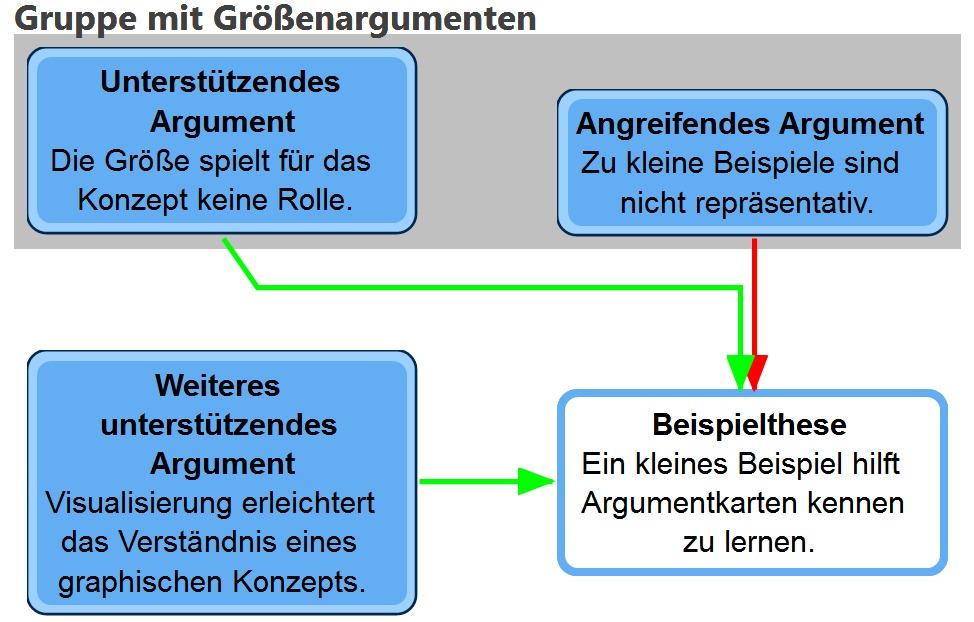
\includegraphics[width=0.5\textwidth]{Pics/Beispielargumentkarte.png}
	\caption{Beispielhafte Argumentkarte mit einer These, drei Argumenten, zwei davon unterstützend und eine angreifend, sowie einer Gruppe.}
	\label{f:Beispielargumentkarte}
\end{center}
\end{figure}

Damit sich die von einer Argumentkarte bereitgestellten Informationen sinnvoll verwenden lassen, muss die Argumentkarte folglich auf eine geeignete Weise dargestellt werden.
Es existieren bereits einige Werkzeuge mit denen Argumentkarten angelegt  und ein Layout automatisch erzeugt werden kann. 
Allerdings müssen die resultierenden Layouts der Argumentkarten oftmals von Hand nachbearbeitet werden, um eine befriedigende Darstellung der Strukturen zu erhalten.
Darüber hinaus ist eine Unterstützung von Gruppen nicht immer gegeben.

% Wie ist diese Ausarbeitung aufgebaut?
%\subsection{Gliederung}
% 1. Problemstellung und -definition
% 2. Lösungsvorschlag
% 3. Detaillierte Erklärung des Algorithmus
% 4. Vergleich zu anderen Lösungsansätzen
In dieser Arbeit geht es um die automatisierte Darstellung von Argumentkarten mit Gruppen, sowie die Interaktion mit diesen Gruppen. Insbesondere hängen diese Gruppen inhaltlich zusammen und werden daher bereits vor der Layouterzeugung festgelegt. Dies ist ein signifikanter Unterschied zu dem oft behandelten Problem des Graphen-Clusterings, bei dem Gruppen als Teil des Layouts auf Basis der Knotenzusammenhänge erzeugt werden.
%und damit um eine Möglichkeit die Argumentkarte zu vereinfachen um dem Benutzer einen schnellen und guten Überblick über die Debatte zu ermöglichen.
Es geht also um die Frage, wie sich Gruppen und Gruppenhierarchien den Anforderungen an Argumentkarten entsprechend visualisieren lassen 
und wie das Layout auf das Öffnen und Schließen von Gruppen reagiert.
%\todo[inline]{Lösungsanstz in Kurzform}

Im nächsten \autoref{chapter:layoutproblem}  präzisieren und abstrahieren wir diese Problemstellung. 
In \autoref{chapter:algo} präsentieren wir unseren Lösungsansatz, welchen wir dann in \autoref{chapter:vgl} mit alternativen Ansätzen vergleichen und bewerten.
\autoref{ch:zsf} schließt mit einer Zusammenfassung.

%-----------------------------------------------------------------------------------------------------------------------------------------------------------------------------------
\chapter{Problemstellung}%\chapter{Layoutproblem} % > mehr als Layout, betrachte auch Interaktion!
\label{chapter:layoutproblem}
In diesem Kapitel definieren wir das von uns behandelte Layoutproblem für Argumentkarten mit Gruppenstruktur, sowie die Anforderungen für Interaktionen mit dem Layout.
Wir beschreiben also wie ein das Layout aussehen soll und was beim Öffnen und Schließen einer Gruppe beachtet werden muss.

\section{Layoutproblem}
\label{sec:layoutproblem}
% Was ist das grundlegende Problem? -> Layout finden
Das Zeichnen eines Graphen setzt sich aus dem Finden eines Layouts sowie des Renderns zusammen. 
Für uns von Interesse ist nur ersteres, das Layoutproblem. 
Ziel hierbei ist es für einen gegebenen Graphen und gegebenenfalls weitere Informationen algorithmisch ein Layout zu berechnen,
welches gewisse Zeichenkonventionen erfüllt, erwünschte Ästhetikkriteren optimiert und gegebenenfalls weiteren lokalen Nebenbedingungen genügt.

% Was macht das Problem speziell? -> Gruppen und dass für Argumentkarten
% Was lässt sich jedoch abstrahieren? -> knoteninhalt, kanten
Im Fall der Argumentkarten abstrahieren wir für das Layoutproblem einige Informationen. 
So spielen die Texte der einzelnen These oder Argumente für uns keine Rolle. 
Sie werden lediglich durch achsenparallele Rechtecke als Knoten des Graphen repräsentiert.
Des Weiteren ignorieren wir bei den Beziehungen zwischen Elementen den Typ sowie die Richtung. 
Es ist also lediglich von Relevanz ob zwei Elemente in einer Beziehung stehen.
Dies wird dann durch eine ungerichtete Kante repräsentiert. 
Eine geschlossene Gruppe wird als Pseudoknoten aufgefasst und durch ein leeres Element repräsentiert.
Dies kann  z.B. ein Rechteck oder ein Kreis sein.  Die Kindgruppen und Knoten einer geschlossenen Gruppe sind folglich verborgen.
Falls auch offene Gruppen dargestellt werden, sollten diese ihre Kindknoten umfassen. 
In einem in \autoref{chapter:vgl} alternativen Ansatz werden offenen Gruppen nicht explizit dargestellt.

Die Eingabe des Algorithmus lässt sich mit diesen Abstraktionen formal beschreiben. 
Sie setzt sich aus einem Graphen $G=(V,E)$, sowie einem Baum $T$, genannt Gruppenbaum,  und einem Schnitt $S$ durch $T$ zusammen. 
Hierbei beschreibt der Gruppenbaum, die Zuteilung von Knoten und Gruppen zu Elterngruppen. 
Der Schnitt gibt den Zustand von Gruppen an, also ob sie geöffnet oder geschlossen sind. Wir spezifizieren nun $T$ und $S$ genauer.

Die Wurzel $r$ der Baumstruktur repräsentiert die ganze Karte, jeder Knoten aus $V$ ist ein Blatt in $T$ und jeder innere Knoten steht für eine Gruppe.
Durch die Distanz eines inneren Knotens zur Wurzel weisen wir die Gruppen einzelnen Stufen zu. 
Da Bäume in der Regel auf dem Kopf gezeichnet werden, bezeichne eine niedrigere Stufe eine höhere Distanz zur Wurzel. Die oberste Stufe sei die Stufe der Wurzel.
%Der Schnitt $S = (X,V \setminus X)$ legt die Menge der derzeitig angezeigten Baumknoten fest 
	% stimmt so nicht, zeigt gruppen an und das haben wir oben genannt
	% außerdem ist V nicht V sondern iwas anderes... geht also nicht so einfach. 
		%daher anstatt overhead einzuführen können wir uns ja darauf verlassen, dass jeder weiß was ein schnitt ist
Für den Schnitt $S$ von $T$ ist gefordert, dass er jeden Pfad von einem Blatt zur Wurzel genau einmal schneidet.
Ein Knoten wird nur angezeigt, wenn der Schnitt den Pfad zur Wurzel von diesem Knoten in der zu diesem Knoten adjazenten Kante schneidet. 
In anderen Worten der Schnitt als \glqq direkt über\grqq\ dem Knoten verläuft.
Eine Gruppe ist geschlossen, also als Pseudoknoten, dargestellt, wenn der Pfad zur Wurzel in der adjazenten Kante geschnitten wird und offen, wenn der Pfad zur Wurzel nicht geschnitten wird. In allen anderen Fällen sind die Knoten oder Gruppen hinter einer geschlossenen Gruppe verborgen und werden nicht angezeigt.
In \autoref{f:LayoutbeispielKlein} wird so ein Layout nach unserem Designkonzept mit dem dazugehörigen Baum und Schnitt dargestellt.

\begin{figure}[h!]
\begin{center} 
  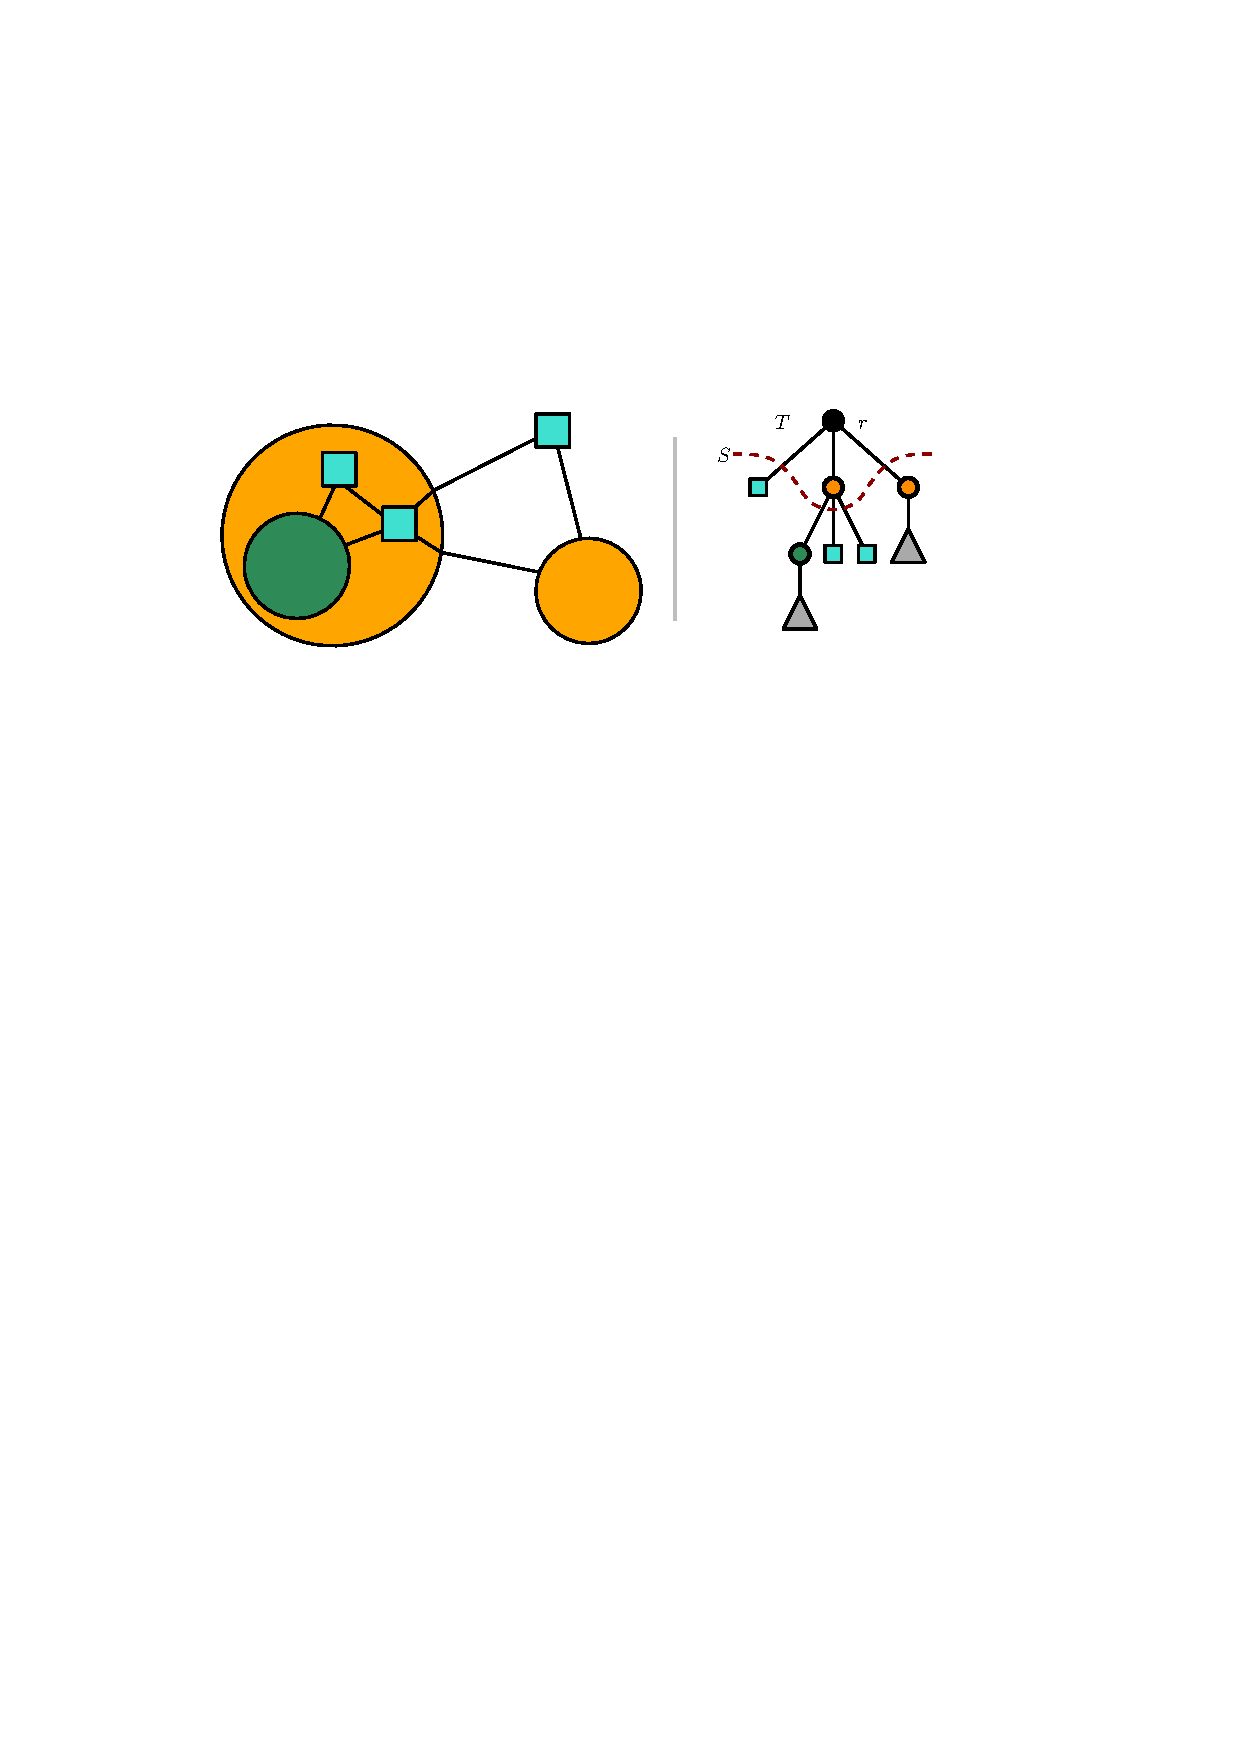
\includegraphics[width=0.6\linewidth]{Pics/LayoutbeispielBaum.pdf}
  \caption{Beispiellayout einer abstrahierten Argumentkarte mit dem dazugehörigen Gruppenbaum und Schnitt. Nicht dargestellte Teilbäume sind im Baum durch graue Dreiecke repräsentiert.}
  \label{f:LayoutbeispielKlein}
\end{center}
\end{figure}

%Die Eingabe des Algorithmus lässt sich mit diesen Abstraktionen formal beschreiben. Sie setzt sich als aus einem Graphen $G=(V,E)$, sowie einem Baum $T$, genannt Gruppenbaum,  und einem Schnitt $S$ durch $T$. Der Gruppenbaum bildet die Knoten auf ihre Gruppen ab.

%Dabei ist der Pseudoknoten $r$ die Wurzel der Baumstruktur, jeder Knoten aus $V$ ist ein Blatt in $T$ und jeder innere Knoten steht für eine Gruppe. 
%Durch die Distanz eines inneren Knotens zur Wurzel weißen wir die Gruppen einzelnen Stufen zu. Da Bäume in der Regel auf dem Kopf gezeichnet werden, bezeichne
%eine niedrigere Stufe eine höhere Distanz zur Wurzel. Die oberste Stufe sei die Stufe der Wurzel.

%Der Schnitt $S = (X,V \setminus X)$ legt die Menge der derzeitig angezeigten Baumknoten fest (Ein Baumknoten ist entweder $r$ ein Gruppe oder ein Knoten aus $G$). Für diese Mengen gilt: $r \in X \setminus V$  und $X \setminus V$ muss ein zusammenhängender Baum sein. Jeder Pfad von $r$ zu einem Wurzelknoten darf also nur einmal geschnitten werden.

%Ein Baumknoten $V^{'}$ wird immer genau dann angezeigt wenn er in $X$ liegt und eine direkte Kante zwischen $V^{'}$ und einem Knoten aus $V \setminus X$ existiert. In anderen Worten: Ein Baumknoten wird immer genau dann angezeigt wenn der Schnitt direkt über dem Knoten verläuft. Falls eine Gruppe in $X$ enthalten ist wird diese durch einen Gruppenknoten abgebildet und ihre Kinder werden nicht angezeigt.

%Dies bedeutet dass ein Knoten oder eine Gruppe nur angezeigt wird wenn er bzw. sie in $S$ enthalten ist.
%Eine Gruppe wird geschlossen, also als Pseudoknoten, dargestellt, wenn der Pfad zur Wurzel in der adjazenten Kante geschnitten wird und offen, wenn der Pfad zur Wurzel nicht geschnitten wird. In allen anderen Fällen sind die Knoten oder Gruppen hinter einer geschlossenen Gruppe verborgen und werden nicht angezeigt.


%Für den Schnitt $S$ von $T$ ist gefordert, dass er jeden Pfad von einem Blatt zur Wurzel genau einmal schneidet.
%Ein Knoten wird nur angezeigt, wenn der Schnitt den Pfad zur Wurzel von diesem Knoten in der zu diesem Knoten adjazenten Kante schneidet. 
%In anderen Worten also direkt über dem Knoten.
%Eine Gruppe wird geschlossen, also als Pseudoknoten, dargestellt, wenn der Pfad zur Wurzel in der adjazenten Kante geschnitten wird und offen, wenn der Pfad zur Wurzel nicht geschnitten wird. In allen anderen Fällen sind die Knoten oder Gruppen hinter einer geschlossenen Gruppe verborgen und werden nicht angezeigt.


%Unter Einbeziehung von Gruppen kann die Eingabe des Algorithmus dann in der Form $G = (V,V_g,E,\sigma)$ dargestellt werden. 
%Die Mengen und Abbildungen dieses Graphen werden im folgenden Beschrieben:
%\todo[inline]{Baumstruktur, Schnitt}
%\todo[inline]{Bulletpoints entfernen}
%\begin{itemize}
%	\item Knoten $V$, Knoten die eine Aussage repräsentieren.
%	\item Gruppenknoten $V_g$, Knoten die eine Gruppe repräsentieren.
%	\item Kanten $E \subseteq \bar{V} \times \bar{V}$, wobei $\bar{V}$ die Menge aller Knoten ($\bar{V} = V \cup V_g$) ist.
%	%\item Rechtseindeutige Abbildung $\lambda(v): V \rightarrow B$, Die Knoten auf die Beschriftungsmenge $B$ (den Text der Knoten) abbildet.
%	 \item Rechtseindeutige Abbildung $\sigma: \bar{V} \rightarrow V_g$, Die Knoten auf ihre Gruppe abbildet (Gruppen können weitere Gruppen enthalten).
%\end{itemize}


Für diese Eingabe definieren wir im folgenden die Zeichenkonventionen und die Ästhetikkriterien des Layoutproblems.

%\section{Formale Beschreibung}\label{sec:formaldesc}
%Eine Argumentkarte lässt sich abbilden auf einen beschrifteten gerichteten Graphen.
%Ein solcher Graph $G = (V, E, \lambda_{v}, \lambda_{e})$ mit Knoten $V$, Kanten $E \subseteq V \times V$, Knotenbeschriftungen $\lambda_{v}:V \rightarrow B_v$ und Kantenbeschriftungen $\lambda_{e}: E \rightarrow B_e$. Dabei sind $B_v$ und $B_e$ die Beschriftungsmengen von Knoten bzw. Kanten.
%Auf einen solchen Graphen lässt sich lässt sich eine Argumentkarte Abbilden wenn die Kantenart als Kantenbeschriftung und der Knotentext als Knotenbeschriftung modelliert wird.
%Gegeben einem solchen beschrifteten gerichteten Graphen kann das Layouten eines Graphen als folgendes Problem modelliert werden:
%\begin{description}\item[Eingabe] \hfill \\[0.3\baselineskip]
%			Beschrifteter gerichteter Graph $G = (V, E, \lambda_{v}, \lambda_{e})$ \hfill \\
			% = \{ \text{achsenparallele Rechtecke}\}
			%sowie einen Gruppenzugehörigkeitsbaum 	
%	\item[Ausgabe] \hfill \\[0.3\baselineskip] Zeichnung mit:
%		\begin{itemize}
%		\item $\forall x,y\in V, x \neq y: x \cap y = \emptyset$, also Knoten paarweise disjunkt
%		\item Überschneidungsfreiheit von Knoten: $\forall x, y \in V: x \neq y \Leftrightarrow x \cap y = \emptyset$
%		\item Überlagerungsfreiheit der Kanten: $\forall x, y \in E: x \neq y \Rightarrow \sigma(x, y) \leq 1$. Wobei $\sigma(x, y): E \times E \rightarrow \mathbb{N}_0$ eine Funktion ist, die für zwei Kanten $x$ und $y$ die Anzahl der Schnittpunkte angibt.
				%$\forall x \in V, (y,z) \in E, y\neq x\neq z: x \cap (y,z) = \emptyset$, also Kanten schneiden nur inzidente Knoten
%		\item Sonstige Nebenbedingung (Layoutanforderungen)
%	\end{itemize}\end{description}


\myparagraph{Zeichenkonventionen}
Zeichenkonventionen beschreiben wie Knoten und Kanten gezeichnet beziehungsweise gelayoutet werden sollen. Sie müssen erfüllt werden.
Für das Layoutproblem von Argumentkarten mit Gruppenstruktur sind dies im Einzelnen:
\begin{itemize}
\item Knoten $V$ werden als achsenparallele Rechtecke dargestellt
\item Überschneidungsfreiheit von Knoten
\item Überschneidungsfreiheit von Kanten mit Knoten
\item Überschneidungsfreiheit von Gruppen mit nicht Kindknoten oder -gruppen, sowie Kanten zwischen solchen
\item Eine geschlossene Gruppe enthält keine Knoten
\end{itemize}

Für unseren Lösungsansatz kommen für Gruppen weitere Zeichenkonvention hinzu. Zum Einen legen wir fest, dass Gruppen
als Kreise dargestellt werden. Zum Anderen fordern wir, dass eine geöffnete Gruppe alle ihre Kindelemente enthält. 
Darüber hinaus spezifizieren wir das Kantenrouting genauer. Dies wird jedoch erst im Lösungsansatz genauer beschrieben.

\myparagraph{Ästhetikriterien}
Ästhetikkriterien sollen vom berechneten Layout optimiert werden. Hauptkriterien sind hier die Größen- und die Kreuzungsminimierung.
Auch wenn es für Argumentkarten im Allgemeinen wünschenswert ist, haben wir in unserem Lösungsansatz die Kreuzungsminimierung nicht beachtet.
Des Weiteren soll sowohl zwischen Knoten als auch Gruppen eine gewisse Mindestdistanz vorhanden sein, sowie Kanten eine gewisse Mindestlänge besitzen.

Lokale Nebenbedingungen haben wir für das Layoutproblem nicht definiert.


%-------------------------------------------------------- INTERAKTION -------------------------------------------------------------
\section{Interaktion mit Gruppen}
% was ist außerdem ein Problem? -> Interkation
Da Gruppen sowohl geöffnet als auch geschlossen sein können, existieren eine Vielzahl von verschiedenen Layouts für eine Argumenkarte.
Jeder gültige Schnitt in $T$ legt eine neue Konfiguration fest und benötigt ein eigenes Layout. 
Das eine Gruppe geöffnet wird bedeutet, dass der neue Schnitt den Gruppenbaum nicht mehr über der Gruppe schneidet, sondern alle seine Kanten zu Kindknoten im Baum.
Das Schließen einer Gruppe wird durch den entgegengesetzten Fall beschrieben. Wir legen zudem fest, dass immer nur eine Gruppe geöffnet oder geschlossen werden kann. Darüber hinaus bezeichnen wir das Öffnen und Schließen einer Gruppe als eine Interaktion.

In einer Implementierung sollte das Wechseln zwischen den verschiedenen Zuständen möglich sein, also der Wechsel des Schnitts und das man eine Gruppe öffnen und schließen kann. 
Dadurch soll es zum einen einfach sein sich einen Überblick zu verschaffen und zum anderen die detailliertere Ansicht zu haben.
% welche Anforderungen haben wir daran? -> nachvollziehbarkeit / beibehalten der mentalen Karte
Hierbei ist es höchst wünschenswert, dass bei einer solchen Interaktion das alte und neue Layout nur so wenig wie möglich und nur so viel wie nötig unterscheiden. 
Positionsänderungen von Knoten und Gruppen sollen bei einer Interaktion nur so groß sein, dass das Layout die Konventionen und Kriterien erfüllt,
Der Nutzer soll sich mit seiner mentalen Karte der Argumentkarte auch nach der Interaktion zurechtfinden können. 
Mit dem Problem, dass bei Veränderungen von Layouts die mentale Karte erhalten bleiben soll, haben sich zum Beispiel schon Eades et. al. \cite{eades1991preserving, Misue1995183}
beschäftigt. Die Anforderung lassen sich auch mit den Konsistenzbedingungen bei dynamischen Kartenbeschriftungen von  Been et. al. \cite{Been2010312} vergleichen.

Eine weitere wünschenswerte Anforderung ist, dass das Layout nach  Auf- und Zuklappzyklen 
wieder zum Anfangslayout oder einem dazu ähnlichem Layout zurückkehrt. 
Ähnlichkeit ist hier so gemeint, dass die Positionsänderungen von Knoten und Gruppen gering sind.

Wir erhalten für eine Interaktion und das Verhältnis der einzelnen berechneten Layouts also weitere Kriterien:
\begin{itemize}
\item Das Layout ändert sich nur so viel wie nötig, um Anforderungen und Kriterien zu genügen. In anderen Worten: Relative Positionen von Elementen verändern sich nur so viel wie nötig.
\item Das Layout zu einem bestimmten Schnitt ist auch nach mehreren Interaktionen das Gleiche oder diesem sehr ähnlich.
\end{itemize}

Von nun an fassen wir die einzelnen Layouts für die verschiedenen Schnitte, also von verschiedenen Zuständen von auf- bzw. zugeklappten Gruppen, nicht mehr einzeln
sondern als ein Layout auf. Ein Wechsel zwischen den einzelnen Layouts nennen wir eine Layoutänderung bei einer Interaktion.

Aus diesen und den in \autoref{sec:layoutproblem} vorgestellten Anforderungen ergibt sich allerdings eine Reihe von Konflikten.
Beispielsweise steht die Größenminimierung der Zeichnung im Konflikt mit der Anforderung, dass sich das Gesamtlayout nur so viel wie nötig ändert, 
da größenminimalere Layouts nach dem Öffnen bzw. Schließen einer Gruppe möglicherweise nur mit einer großen Veränderung des Layouts möglich sind.
Der im Folgenden präsentierte Ansatz schlägt jedoch Problemlösungen vor oder präferiert eine der Optionen.

%\todo[inline]{Zusammenhang der Probleme hervorheben. Interkation hat Einfluss auf Wahl des Layouts, etc.}
